\documentclass[10pt,a4paper]{ctexart}
\usepackage[margin=1.6cm]{geometry}
\usepackage{graphicx,booktabs,amsmath,caption,float,hyperref}
\usepackage{titlesec}
\setlength{\parskip}{3pt}
\setlength{\parindent}{1em}
\titlespacing*{\section}{0pt}{4pt}{2pt}
\titlespacing*{\subsection}{0pt}{3pt}{1pt}
\captionsetup{font=small,labelfont=bf}
\begin{document}
\begin{center}
{\Large \bfseries 基于 MyoKi 人手运动学数据的抓取姿态协同统计分析}\\[4pt]
{\normalsize 生物统计和生物信息引论 Final Project}\\[2pt]
\end{center}
\noindent\textbf{摘要} 本项目将人手抓取姿态协同分析组织为一个统计问题：MyoKi 抓取运动学中是否存在稳定的低维协同结构，该结构是否能解释抓取家族差异，并且是否能跨受试者预测。分析纳入 23 名右利手健康受试者、41 个抓取任务和 5656 个试次。主成分分析作为表征层，后续加入受试者 bootstrap、方差解释复杂度指数（Variance-Accounted-For Complexity Index, VAF-CI）、受试者 blocked ANOVA、Benjamini-Hochberg 假发现率校正和留一受试者交叉验证。前两个主成分解释 91.0\% 任务级方差，整体 VAF-CI 为 0.030，达到 90\% 方差解释率需要 2 个主成分。\\
\textbf{关键词} 手部运动学；姿态协同；主成分分析；bootstrap；blocked ANOVA；逻辑回归

\section{数据来源与研究问题}
MyoKi 数据集由 CyberGlove II 记录健康受试者在日常生活操作中的手部运动学信号。数据从公开发布网站下载后，按试次边界截取 CyberGlove II 手部关节角时间序列，并通过线性插值把每个试次重采样到 100 帧；随后剔除掌弓通道和两个腕部通道，保留 15 个手指相关关节通道。根据 \texttt{Task\_categorization.xlsx} 筛选 41 个抓取任务，并将任务归并为力量型、精细型和复杂型三个抓取家族。研究问题为：1）抓取姿态变化能否由少数协同轴解释；2）方差集中度和 VAF-CI 是否表明任务需要不同程度的个体化关节控制；3）不同抓取家族在协同空间中是否存在统计差异；4）低维协同是否保留预测抓取类别的信息。

\section{研究方法}
对每个试次计算 15 个关节的角度活动范围 $\max(\theta_j)-\min(\theta_j)$，得到试次级特征。主成分分析在任务均值矩阵上拟合，以避免重复试次数量主导协方差结构；随后将每个试次投影到同一协同空间。参考 West 等人的方差解释复杂度指数，本研究从累计方差解释曲线计算 VAF-CI：当更多主成分才能解释同样比例的方差时，说明该任务家族需要更强的关节个体化控制。

统计推断包括四部分。首先，以受试者为重采样单位进行 1000 次 bootstrap，估计方差解释率和 VAF-CI 的 95\% 置信区间。其次，分别计算三个抓取家族的 VAF-CI 和达到 90\% 方差解释率所需的主成分数。第三，以主成分得分为因变量，用受试者固定效应进行 blocked ANOVA：$\mathrm{PC} \sim \mathrm{grasp\ family} + \mathrm{subject}$。两两比较使用 Benjamini-Hochberg 假发现率校正。第四，使用留一受试者交叉验证训练多项逻辑回归，比较原始 15 维特征、前 2、3、5 个主成分对抓取家族的预测能力。

\section{主要结果}
任务级主成分分析显示，第一主成分解释 78.0\% 方差，第二主成分解释 13.0\%，前两维合计 91.0\%。受试者 bootstrap 得到前两主成分方差解释率 95\% 置信区间为 [89.1\%, 91.4\%]。VAF-CI 分析显示，整体数据的 VAF-CI 为 0.030；力量型、精细型和复杂型抓取的 VAF-CI 分别为 0.022、0.031 和 0.009。

受试者 blocked ANOVA 显示，抓取家族对第一主成分的影响显著（F(2, 5631)=300.1, p=1.4e-124, 偏 $\eta^2$=0.096），对第二主成分亦显著（F(2, 5631)=1137.0, p=$<10^{-300}$, 偏 $\eta^2$=0.288）。留一受试者交叉验证显示，最佳方案为 Raw15，平衡准确率为 0.70$\pm$0.09。

\section{图表}
\begin{figure}[H]\centering
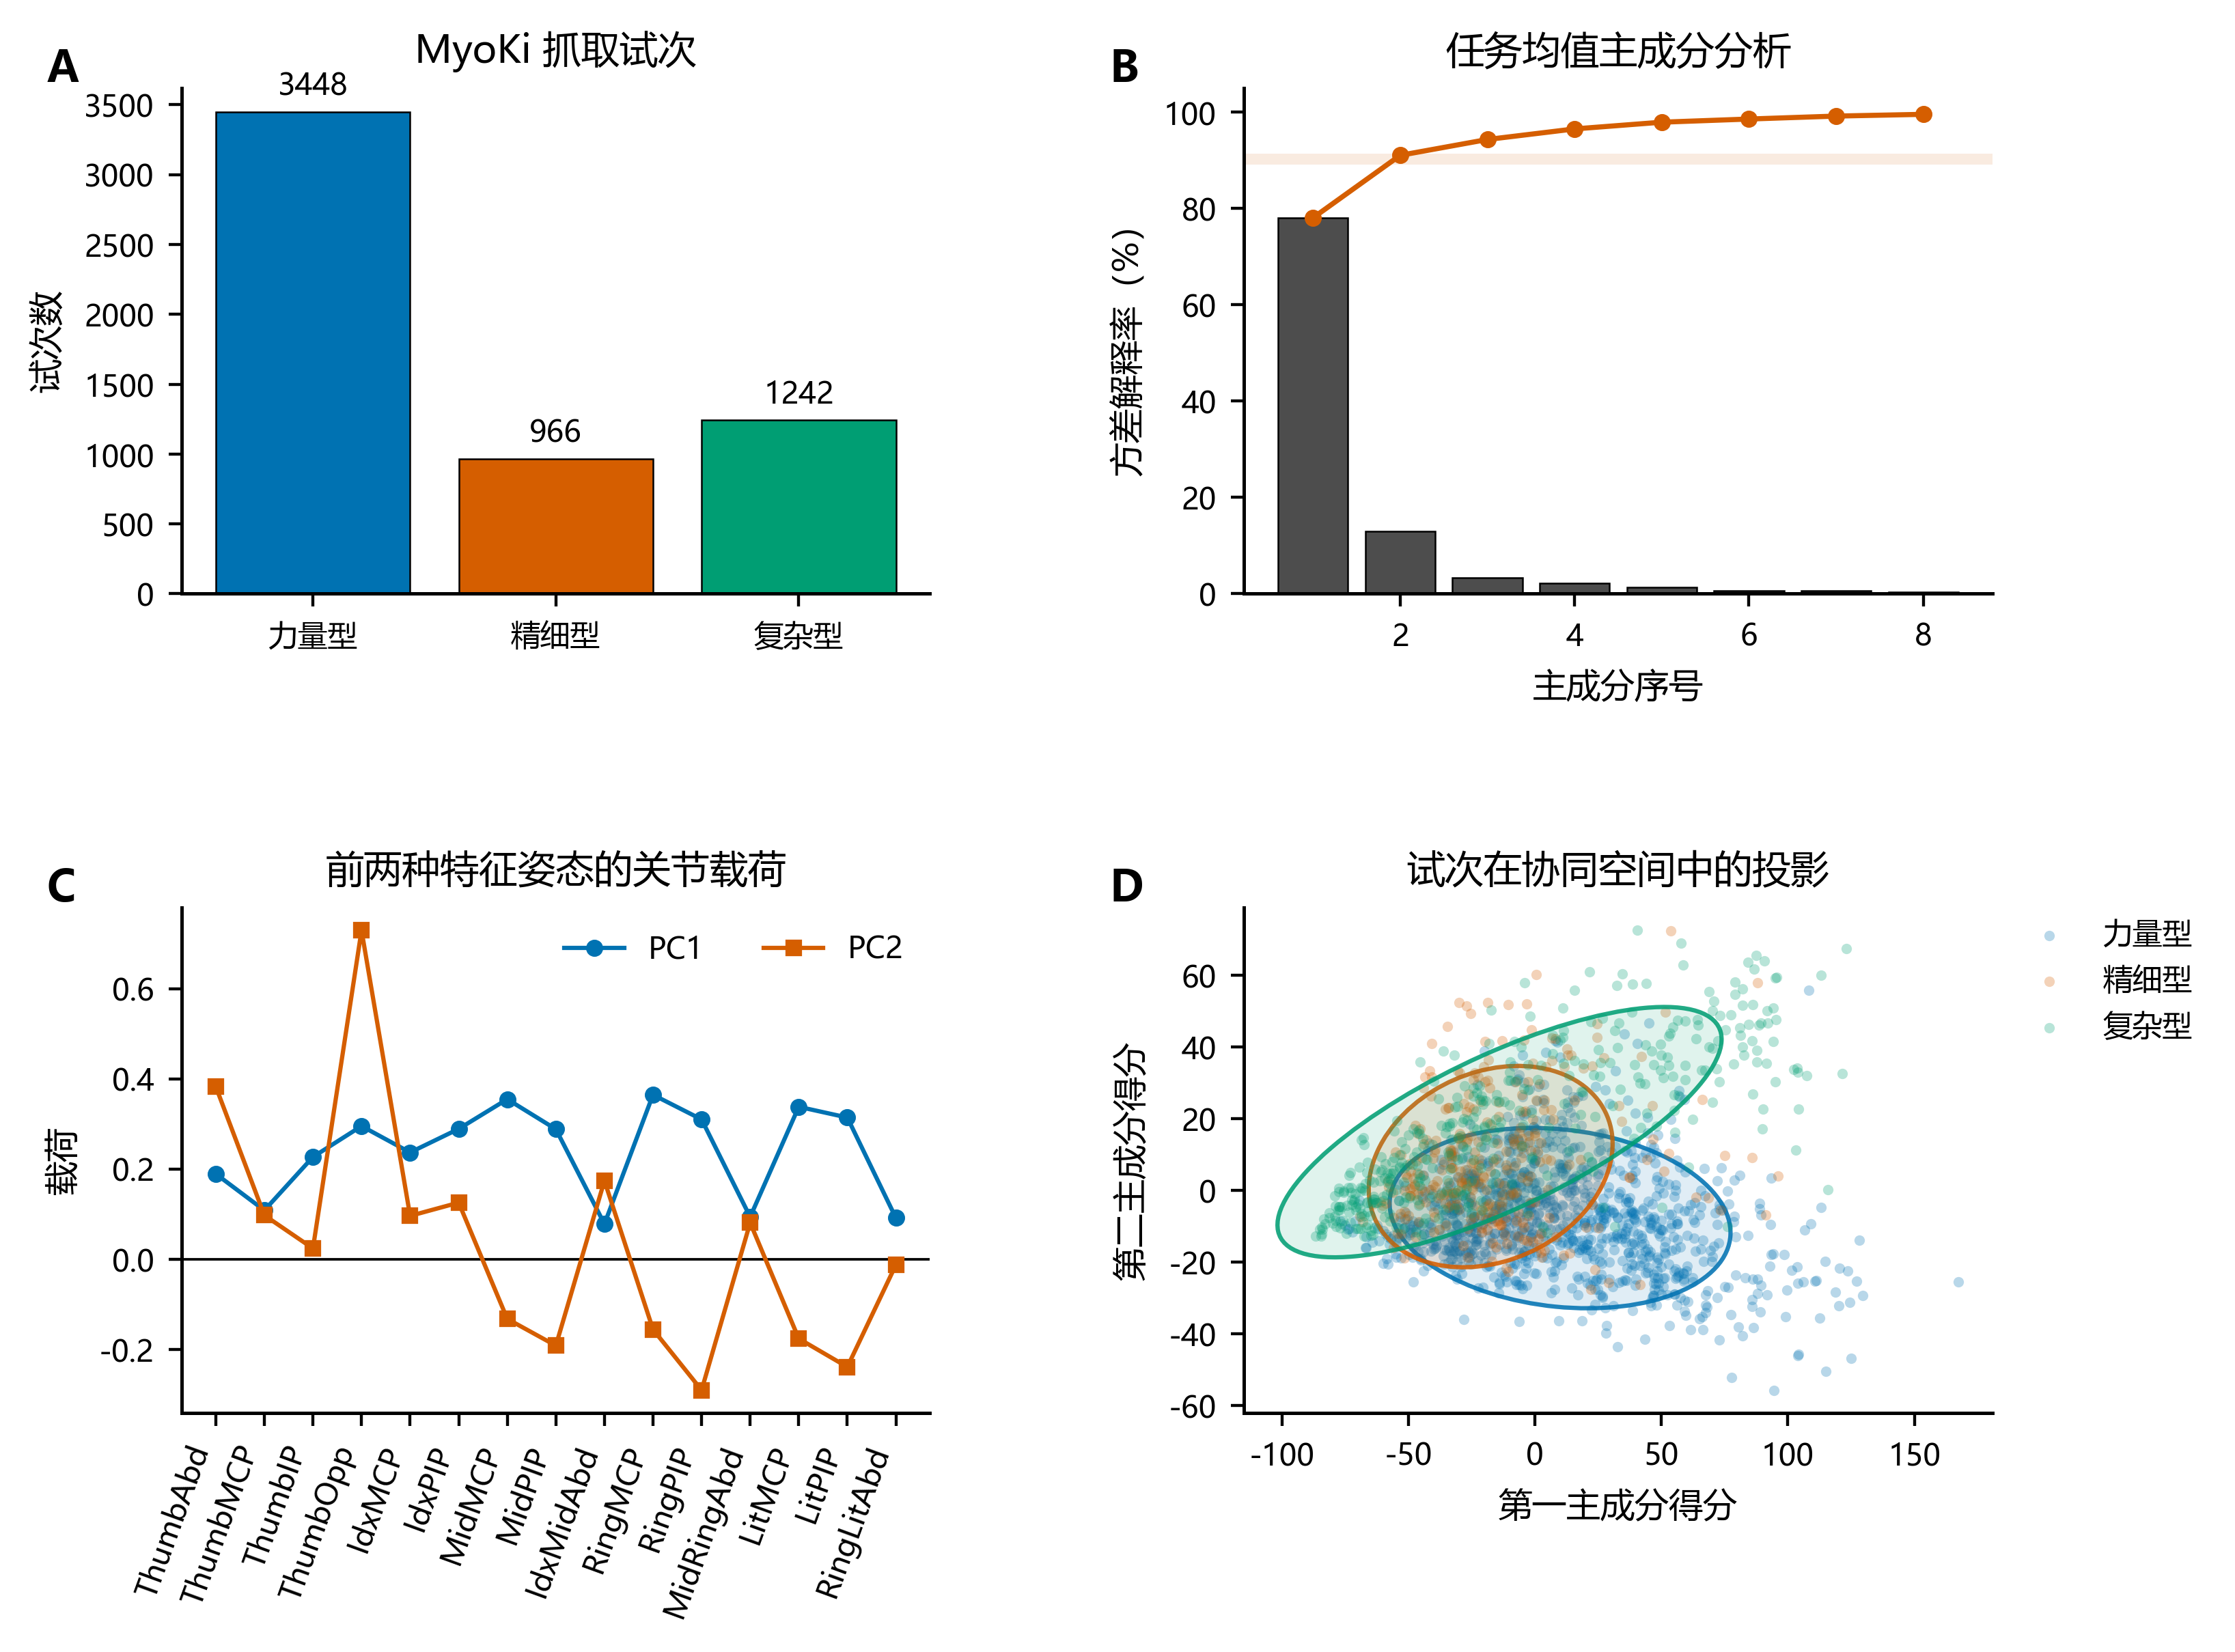
\includegraphics[width=0.88\linewidth]{../outputs/figures/figure1_pca_overview.png}
\caption{数据结构、任务级主成分分析、关节载荷与试次投影。}
\end{figure}
\begin{figure}[H]\centering
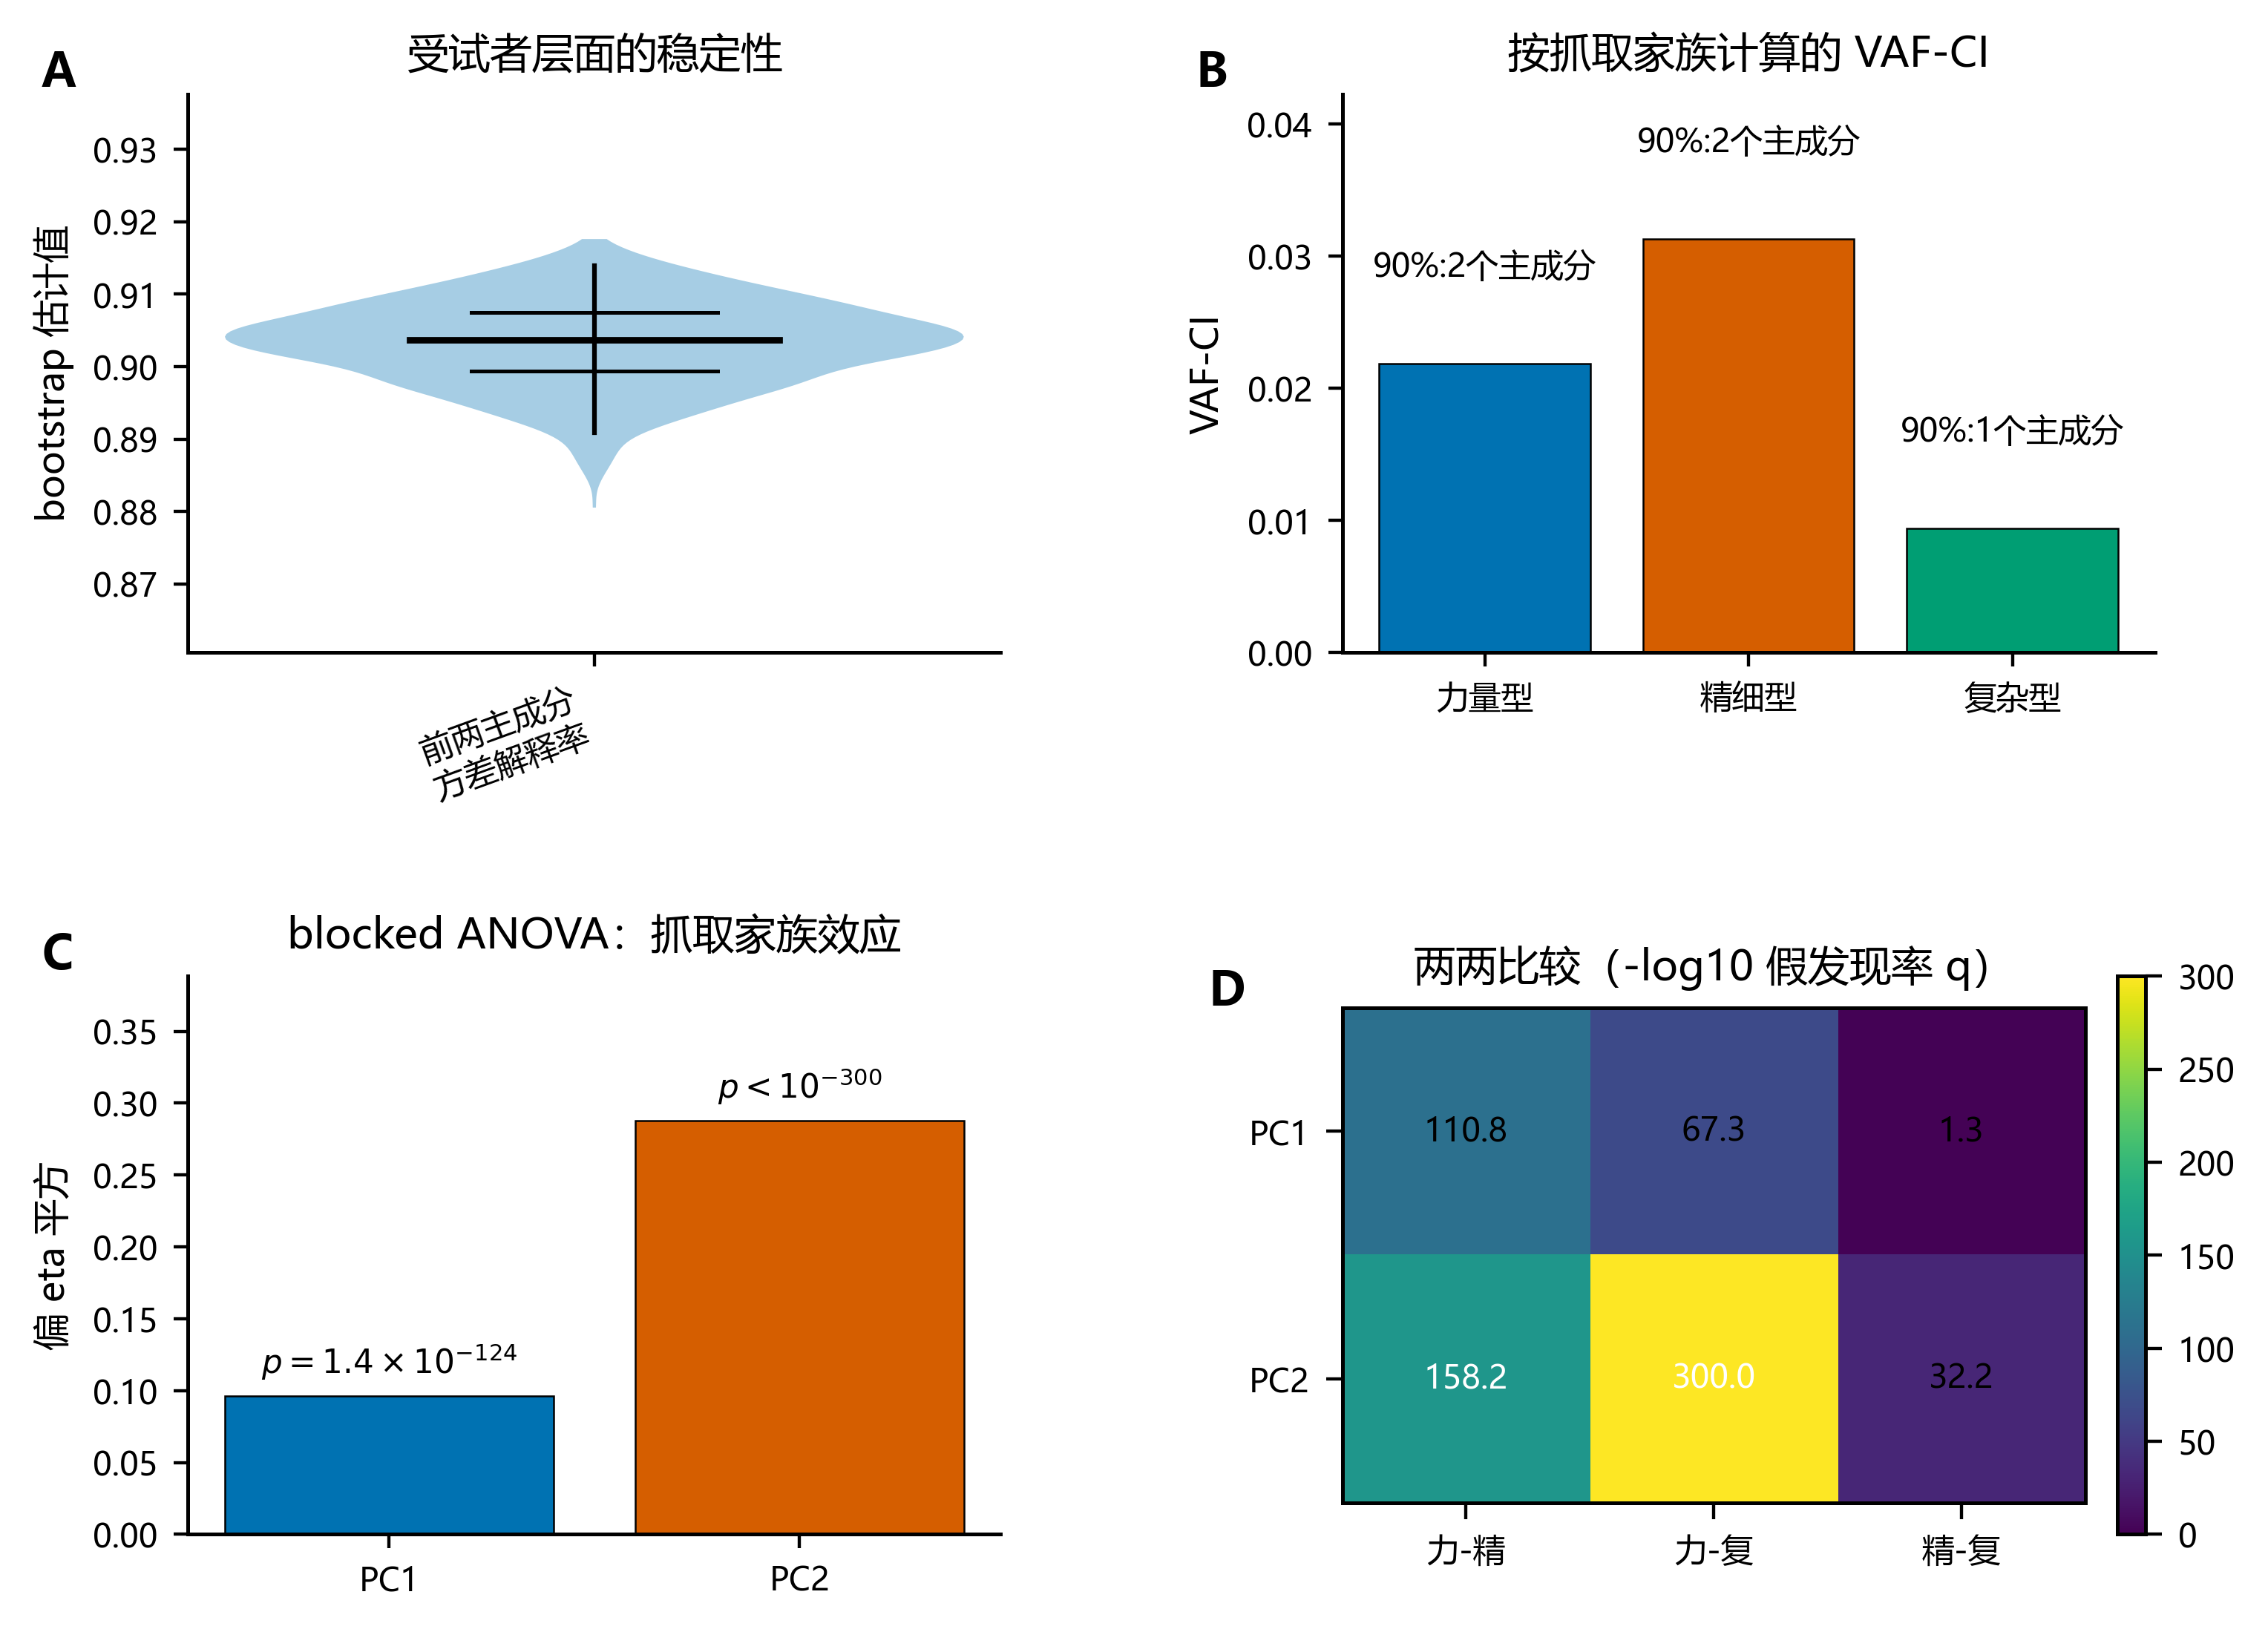
\includegraphics[width=0.88\linewidth]{../outputs/figures/figure2_inference.png}
\caption{bootstrap、VAF-CI、blocked ANOVA 和 FDR 校正的两两比较。}
\end{figure}
\begin{figure}[H]\centering
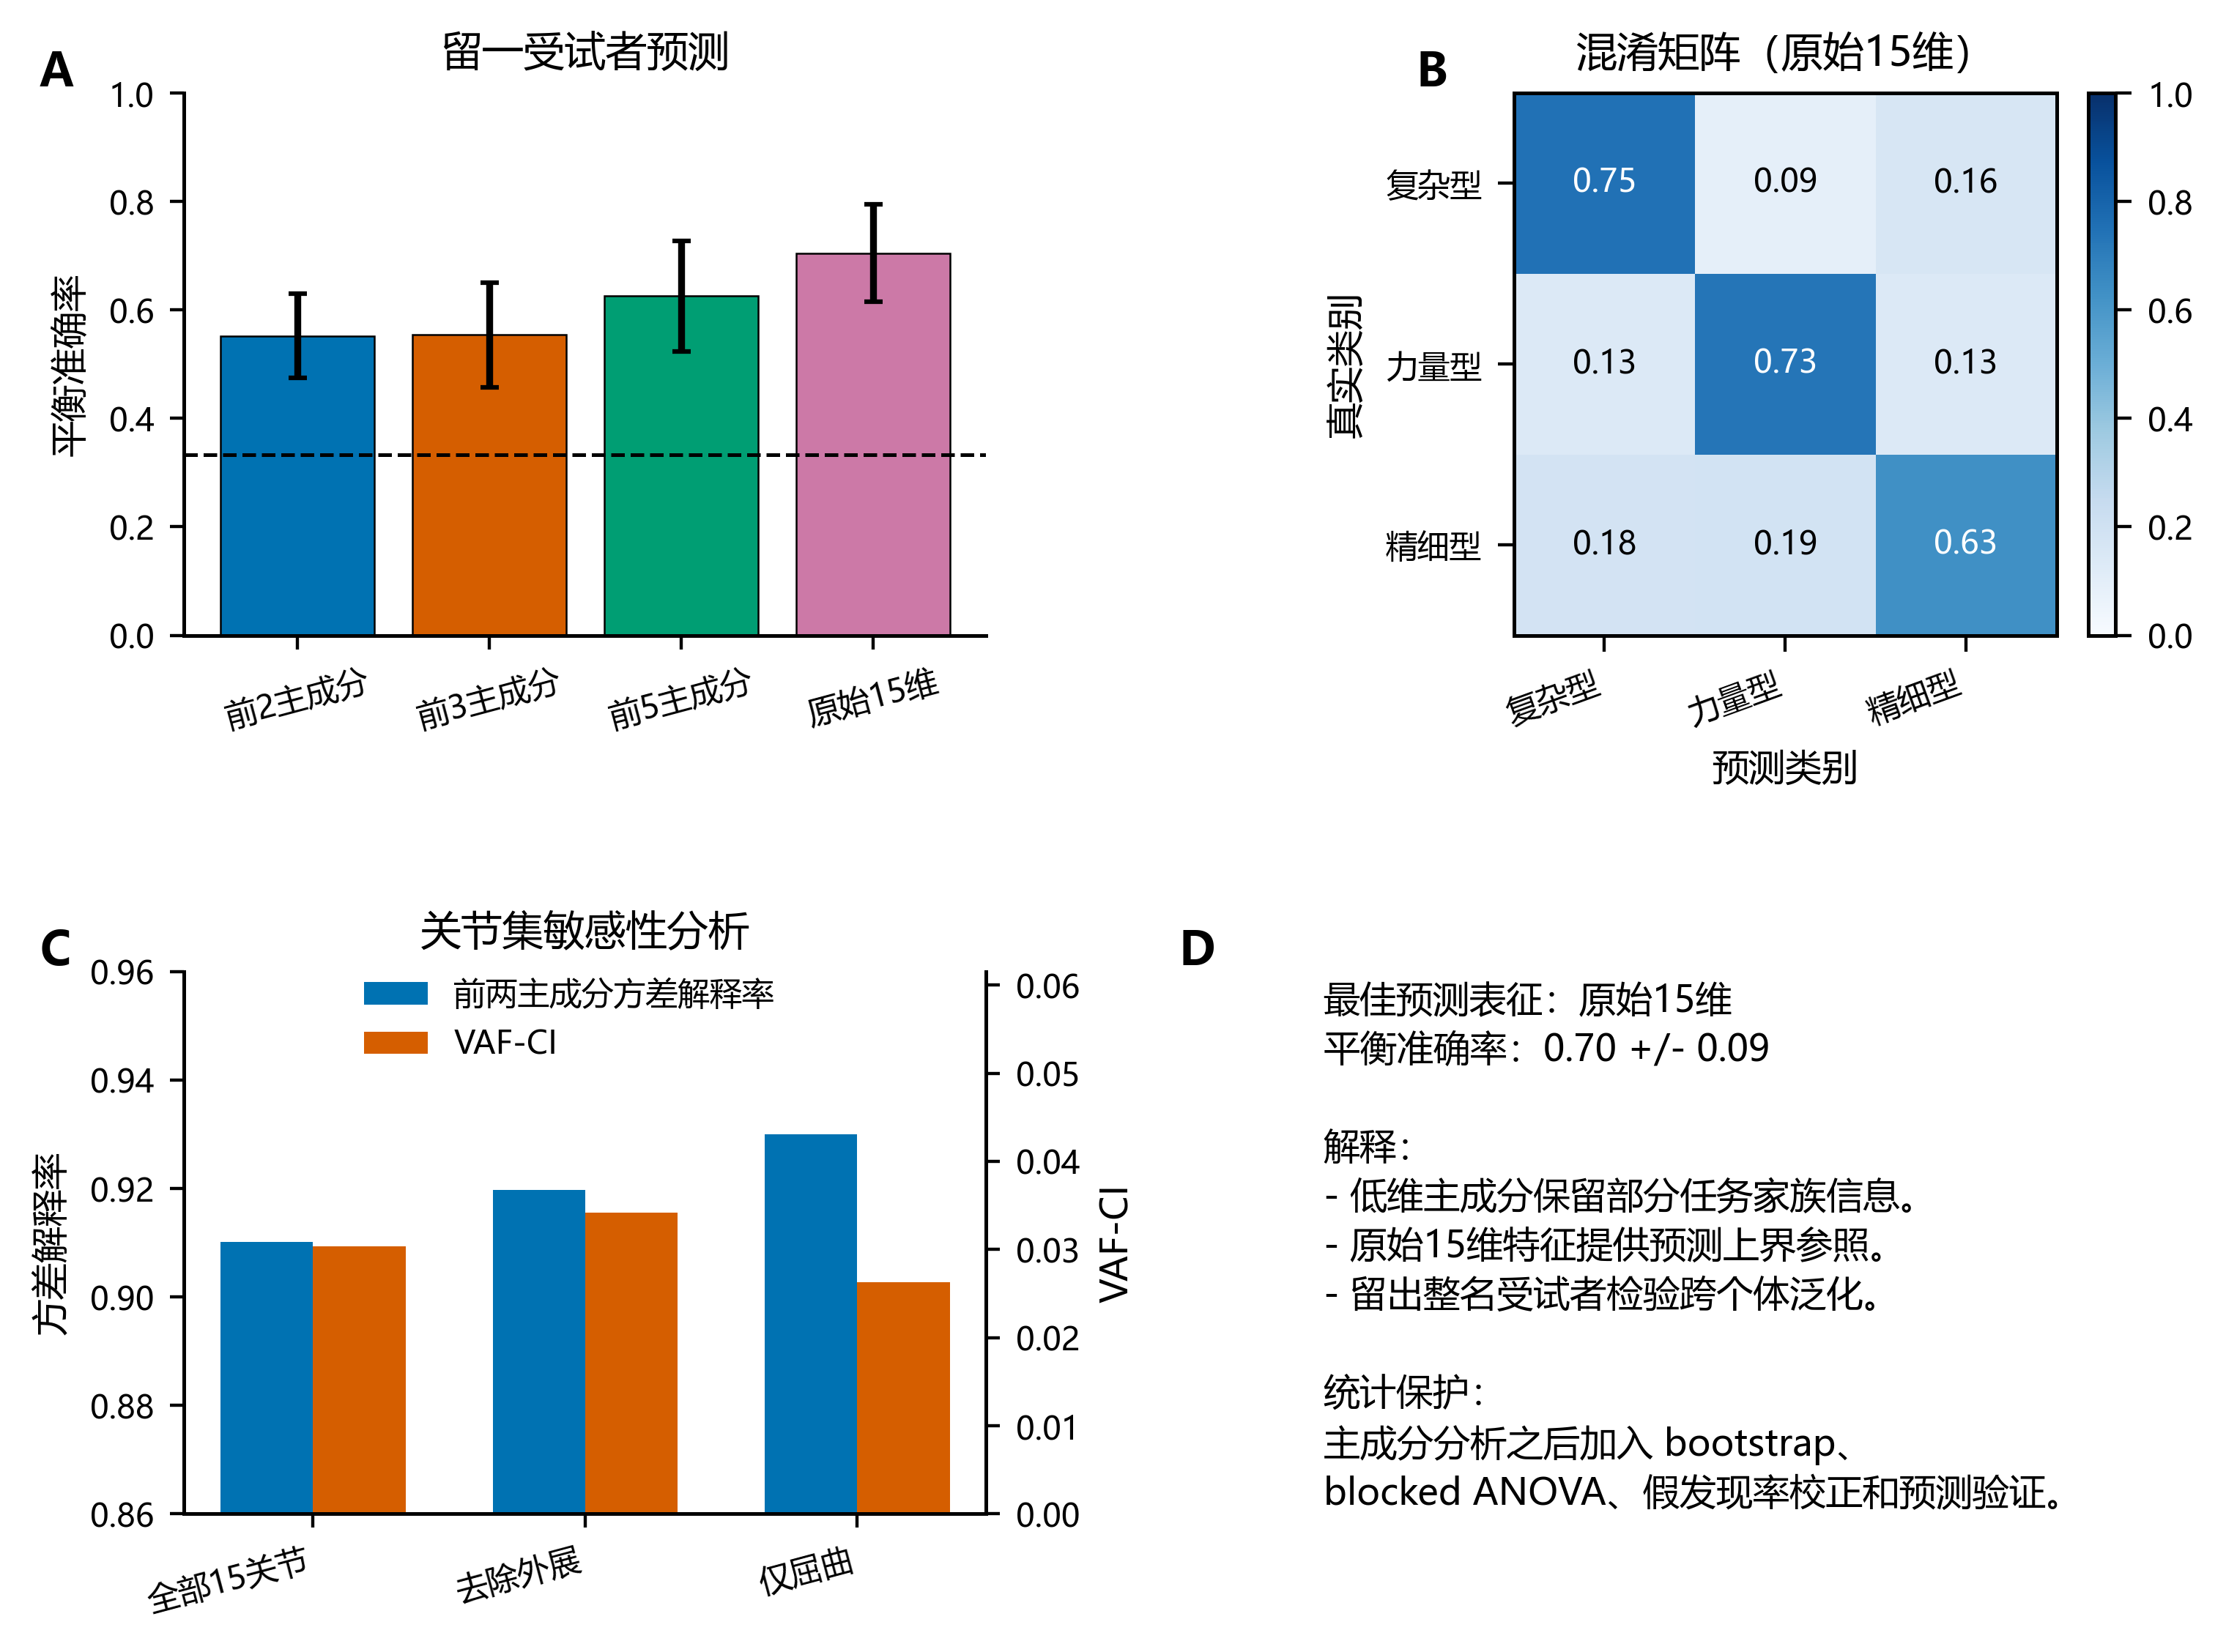
\includegraphics[width=0.88\linewidth]{../outputs/figures/figure3_prediction_sensitivity.png}
\caption{留一受试者预测验证、混淆矩阵和关节集敏感性分析。}
\end{figure}

\section{结论与局限性}
本项目支持一个统计上更完整的结论：人手抓取运动学中存在稳定的低维姿态协同结构。主成分分析将 15 维运动学数据转化为可解释表征；bootstrap 量化不确定性，VAF-CI 描述方差集中度，blocked ANOVA 检验任务差异，逻辑回归验证预测价值。局限性包括：健康受试者数据不能直接推广至神经损伤或假肢用户；角度活动范围忽略了完整时间序列的相位和速度信息；主成分分析是线性方法；预测验证基于现有任务标签，不能替代真实控制系统或临床性能评估。

\section{参考文献}
\begin{enumerate}\setlength\itemsep{2pt}
\item Santello M, Flanders M, Soechting JF. Postural hand synergies for tool use. \emph{Journal of Neuroscience}. 1998;18(23):10105-10115.
\item Jarque-Bou NJ, et al. A database of multimodal myography and hand kinematics during realistic daily life activities. \emph{Scientific Data}.
\item Feix T, Romero J, Schmiedmayer H-B, Dollar AM, Kragic D. The GRASP taxonomy of human grasp types. \emph{IEEE Transactions on Human-Machine Systems}. 2016;46(1):66-77.
\item West AM, Tessari F, Wang M, Hogan N. The Study of Dexterous Hand Manipulation: A Synergy-Based Complexity Index. \emph{IEEE Transactions on Medical Robotics and Bionics}. 2025;7(1):156-163.
\end{enumerate}

\section*{复现说明}
代码入口：\texttt{course\_project/scripts/run\_course\_final\_analysis.py}；课程论文构建：\texttt{course\_project/scripts/build\_course\_paper.py}。本科毕业论文中的协同分析章节仅用于理解项目背景，未列入参考文献。
\end{document}
